\documentclass{article}

\usepackage[utf8]{inputenc}
\usepackage{titlesec}
\usepackage{easylist}
\usepackage{hanging}
\usepackage{hyperref}
\usepackage[a4paper,top=2.0cm,bottom=2.0cm,left=2.0cm,right=2.0cm]{geometry}
\usepackage{blindtext}
\usepackage{tipa}
\usepackage{epigraph}
\usepackage{enumerate}
\usepackage{longtable}
\usepackage{setspace}
\usepackage{verbatim}
\usepackage[T1]{fontenc}
\usepackage{graphicx}
\usepackage[italian]{babel}
\usepackage{amsmath}
\usepackage{pbox}
\usepackage{fancyhdr}
\usepackage{cancel}
\usepackage{tabularx}
\usepackage{booktabs}
\usepackage{multirow}
\usepackage{longtable}
\usepackage{tikz}
\usepackage{tikz-qtree}
\usepackage{subfig}
\usepackage{xcolor}
\usepackage{amssymb}
\usepackage{mathrsfs}
\usepackage{textcomp}

\usepackage{listings}
\usepackage{color}

% Teoremi
\newtheorem{notab}{Nota bene}

\definecolor{mygreen}{rgb}{0,0.6,0}
\definecolor{mygray}{rgb}{0.5,0.5,0.5}
\definecolor{mymauve}{rgb}{0.58,0,0.82}

\lstset{ 
  backgroundcolor=\color{white},   % choose the background color; you must add \usepackage{color} or \usepackage{xcolor}; should come as last argument
  basicstyle=\footnotesize,        % the size of the fonts that are used for the code
  breakatwhitespace=false,         % sets if automatic breaks should only happen at whitespace
  breaklines=true,                 % sets automatic line breaking
  captionpos=b,                    % sets the caption-position to bottom
  commentstyle=\color{mygreen},    % comment style
  deletekeywords={...},            % if you want to delete keywords from the given language
  escapeinside={\%*}{*)},          % if you want to add LaTeX within your code
  extendedchars=true,              % lets you use non-ASCII characters; for 8-bits encodings only, does not work with UTF-8
  firstnumber=1000,                % start line enumeration with line 1000
  frame=single,	                   % adds a frame around the code
  keepspaces=true,                 % keeps spaces in text, useful for keeping indentation of code (possibly needs columns=flexible)
  keywordstyle=\color{blue},       % keyword style
  language=Octave,                 % the language of the code
  morekeywords={*,...},            % if you want to add more keywords to the set
  numbers=left,                    % where to put the line-numbers; possible values are (none, left, right)
  numbersep=5pt,                   % how far the line-numbers are from the code
  numberstyle=\tiny\color{mygray}, % the style that is used for the line-numbers
  rulecolor=\color{black},         % if not set, the frame-color may be changed on line-breaks within not-black text (e.g. comments (green here))
  showspaces=false,                % show spaces everywhere adding particular underscores; it overrides 'showstringspaces'
  showstringspaces=false,          % underline spaces within strings only
  showtabs=false,                  % show tabs within strings adding particular underscores
  stepnumber=2,                    % the step between two line-numbers. If it's 1, each line will be numbered
  stringstyle=\color{mymauve},     % string literal style
  tabsize=2,	                   % sets default tabsize to 2 spaces
  title=\lstname                   % show the filename of files included with \lstinputlisting; also try caption instead of title
}

\linespread{1.5} % l'interlinea

\frenchspacing

\newcommand{\abs}[1]{\lvert#1\rvert}

\usepackage{floatflt,epsfig}

\usepackage{multicol}
\newcommand\yellowbigsqcup[1][\displaystyle]{%
  \fboxrule0pt
  \ifx#1\textstyle\fboxsep-0.6pt\else\fboxsep-1.25pt\fi
  \mathrel{\fcolorbox{white}{yellow}{$#1\bigsqcup$}}}

\title{Rudimenti di Matematica: \\ {\large\it Polinomi e prodotti notevoli}}
\author{Nicola Ferru}
\begin{document}
\maketitle

\section{Monomio}
\label{sec:monomio}

Un monomio è un'espressione algebrica costituita da un coefficiente e una parte letterale dove tra le lettere
compaiono moltiplicazione e elevamenti a potenza aventi esponente naturale\footnote{Numero naturale =
numeri che vengono utilizzati per contare o ordinare, senza virgola.}. Ad esempio
\begin{eqnarray}
  \label{eq:monomi}
  2x; & -x^n; & x^2y
\end{eqnarray}
\begin{notab}
  In caso di esponente pari il monomio anche se con segno negativo, nello sviluppo cambierà segno diventando
  positivo.
\end{notab}
\section{Binomio}
\label{sec:binomio}

In matematica i binomi vengono definiti come la somma di due monomi.
\begin{equation}
  \label{eq:a+b}
  (a+b)
\end{equation}
Ogni lettera indica sempre un \underline{numero reale} o \underline{complesso},
le variabili sono scritte sempre in minuscolo, al contrario delle costanti che, che invece,
vanno sempre in maiuscolo.
\subsection{Quadrato}
\label{sec:binomiodi2}
Il quadrato di un binomio si svolge nel seguente modo:
\begin{eqnarray}
  \label{eq:quadratodibinomio}
  (a+b)^2=a^2+b^2+2ab & \to & a^2+2ab+b^2
\end{eqnarray}
\begin{figure}[th]
  \centering
  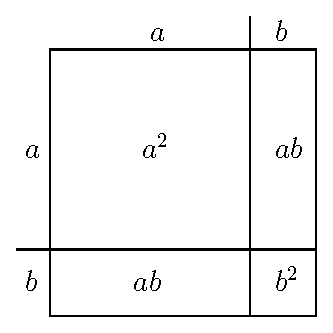
\includegraphics[width=4cm]{img/binomio.eps}
  \caption{dimostrazione grafica dell'identità}
  \label{fig:identità}
\end{figure}
\begin{notab}
  Quando l'esponente è pari i due prodotti sono sempre positivi, mentre, i doppi prodotti risentono del segno
  del polinomio di origine. Ad esempio:
  \begin{eqnarray}
    \label{eq:quadratodibinomioconsegnonegativo}
    (a-b)^2=a^2+b^2-2ab & \to & a^2-2ab+b^2
  \end{eqnarray}
\end{notab}
Ma prendiamo un caso reale per poter constatare gli effetti reali dello sviluppo, infatti, andremo a sostituire
$a$ e $b$ con dei un valore e un incognita.
\begin{equation*}
  (x+3)^2=x^2 + 9 + 6x
\end{equation*}
Andando a riordinarla per grado di $x$ il risultato finale sarà: $x^2+6x + 9$

\subsection{Cubo}
\label{sec:qudodibinomio}

Il cubo di binomio è composto dal cubo del primo monomio, più il triplo del prodotto del quadrato del primo
monomio per il secondo, più il triplo del prodotto del primo monomio per il quadrato del secondo, più il cubo
del secondo monomio. Quindi lo svolgimento sarà il seguente:
\begin{eqnarray}
  \label{eq:cubodibinomio}
  (a+b)^3=a^3+b^3+3a^2b+3ab^2 & \to & a^3+3a^2b+3ab^2+b^3
\end{eqnarray}
mentre, nel caso in cui il segno del secondo monomio risulti essere negativo, il risultato finale sarà:
\begin{eqnarray}
  \label{eq:cubodibinomioneg}
  (a-b)^3=a^3-b^3-3a^2b+3ab^2 & \to & a^3-3a^2b+3ab^2-b^3
\end{eqnarray}
Come nel caso precedente (\ref{eq:quadratodibinomio}) andiamo a sostituire $a$ e $b$ con dei valori e delle
costanti:
\begin{eqnarray*}
  (x+2)^3=x^3+8+6x^2+12x & \to  & x^3+6x^2+12x+8
\end{eqnarray*}
\subsection{Esponente superiore al 3}
Nel caso in cui il binomio viene elevato con un valore superiore al 3 la formula che viene applicata è la
seguente:
\begin{equation}
  \label{eq:binomioformelev}
  (a+b)^n=a^n+C_{n,1}a^{n-1}b+C_{n,2}a^{n-2}b^2+\dots+C_{n,n-1}ab^{n-1}+b^n
\end{equation}
devo i $C_{n,1}a^{n-1}b,C_{n,2}a^{n-2}b^2,\dots$ sono i coefficienti binomiali ottenibili tramite il Triangolo di
Tartaglia.\\
Facciamo un l'esempio, prendiamo un binomio elevendolo per 4, infatti, in questo caso lo sviluppo sarà il
seguente:
\begin{equation}
  \label{eq:polquartogrado}
  (a+b)^4=a^4 + 4a^3b+6a^2b^2+4ab^3+b^4
\end{equation}

\subsection{Scomposizione di un binomio}
\label{sec:scomposizionebin}
Per scomporre un binomio il metodo più semplice è il seguente:
\begin{enumerate}
\item Si mette in evidenza il fattor comune;
\item Si divide per il fattor comune;
\item se può essere ulteriorimente diviso lo si divide in due binomi, più il monomio che ne rimaneva dal fattor
  comune.
\end{enumerate}
Ad esempio
\begin{equation}
  \label{eq:scomposizionebin}
  \frac{5}{4}b-125b^3
\end{equation}
Per prima cosa andiamo a cercare il fattor comune, che in questo caso è $5b$ e lo mettiamo in evvidenza
\begin{equation*}
  =5b\cdot\left(\frac{1}{4}-25b^2\right)
\end{equation*}
Visto che all'interno delle parendesi tonde e ancora presente un grado due quindi può essere ulteriormente
separato effettuiamo la seguente separazione:
\begin{equation*}
  5b\cdot \left(\frac{1}{2} + 5b\right)\left(\frac{1}{2}-5b\right)
\end{equation*}
Quindi il risultato finale è composto da un monomio e un prodotto tra binomi.
\clearpage
\subsubsection{Il triangolo di Tartaglia}
\label{sec:tartaglia}
\begin{table}[th]
  \centering
  \begin{tabular}{>{$n=}l<{$\hspace{12pt}}*{13}{c}}
    0 &&&&&&&1&&&&&&\\
    1 &&&&&&1&&1&&&&&\\
    2 &&&&&1&&2&&1&&&&\\
    3 &&&&1&&3&&3&&1&&&\\
    4 &&&1&&4&&6&&4&&1&&\\
    5 &&1&&5&&10&&10&&5&&1&\\
    6 &1&&6&&15&&20&&15&&6&&1
  \end{tabular}
  \caption{Triangolo di Tartaglia}
  \label{tab:tartagliagr}
\end{table}
Il triangolo di Tartaglia ({\it anche detto triangolo di pascal}) è una delle disposizione geometrica dei
coefficienti binomiali, ossia dei coefficienti di sviluppo del binomio (\ref{sec:binomio}) elevato a una
qualsiasi potenza $n$, a forma di triangolo.

\section{Trinomio}
\label{sec:trinomio}
Un trinomio è un polinomio composto da tre termini; in altre parole una somma tra tre monomi. Ad esempio $a+b+c$.
\begin{equation}
  \label{eq:trinomio}
  (x-x_1)(x-x_2)
\end{equation}
dove $x_1$ e $x_2$ sono due numeri reali tali che: $x_1+x_2=s$ e $x_1x_2=p$.

\end{document}
